\begin{figure}
  \centering
  \begin{subfigure}[t]{0.28\textwidth}
    \centering
    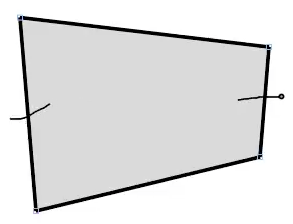
\includegraphics[width=40mm]{img/same-length-1.png}
    \caption{Same Length gesture.}
    \label{fig:same-length-1}
  \end{subfigure}
  \hspace{1cm} % spacing, do what you need
  \begin{subfigure}[t]{0.28\textwidth}
    \centering
    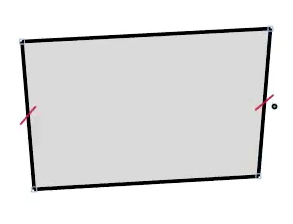
\includegraphics[width=40mm]{img/same-length-2.png}
    \caption{After recognition.}
    \label{fig:same-length-2}
  \end{subfigure}
  \hspace{1cm} % spacing, do what you need
  \begin{subfigure}[t]{0.28\textwidth}
    \centering
    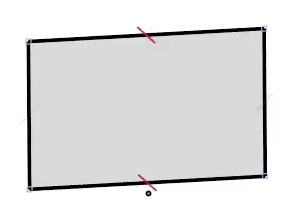
\includegraphics[width=40mm]{img/same-length-3.png}
    \caption{A second constraint.}
    \label{fig:same-length-3}
  \end{subfigure}

  \vspace{5mm}
  \begin{subfigure}[t]{0.35\textwidth}
    \centering
    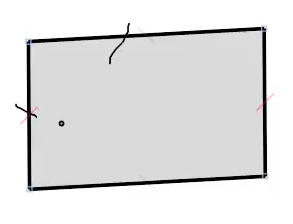
\includegraphics[width=40mm]{img/same-length-4.png}
    \caption{Combining constraints.}
    \label{fig:same-length-4}
  \end{subfigure}
  \hspace{1cm} % spacing, do what you need
  \begin{subfigure}[t]{0.35\textwidth}
    \centering
    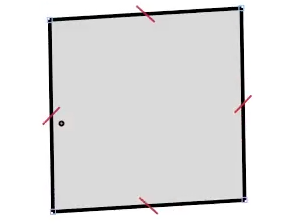
\includegraphics[width=40mm]{img/same-length-5.png}
    \caption{Result is a rhombus.}
    \label{fig:same-length-5}
  \end{subfigure}

  \caption[Same Length constraints]{Examples of making two separate
    Same Length constraints, then combining them into a single Same
    Length constraint.}
  \label{fig:same-length}
\end{figure}
